\subsection{要求管理活動}

要求開発が「合意を作る活動」だとすれば、\term{要求管理}は「合意を維持する活動」である。要求は開発中にも保守中にも変わる。したがって、不要な要求を減らし、変更を統制し、範囲と制約を整合させる必要がある。

\subsubsection{要求整理・削減}

\term{要求整理・削減}は、英語の \,\en{Requirements Scrubbing}\, に対応する。目的は、利害関係者のニーズを満たすために必要な、できるだけ小さく、単純な要求集合を得ることである。

削減の対象は、範囲外の要求、費用対効果が低い要求、重要度が低い要求、過度に複雑な要求である。要求が減れば、設計、実装、テスト、保守の負担も減る。

\subsubsection{要求変更管理}

\term{要求変更管理}とは、合意済みの要求を変更する手順を管理する活動である。計画駆動型の開発では、変更要求、影響分析、承認・却下・保留の判断、関係者への通知、完了までの追跡が明示的に行われることが多い。

アジャイル型の開発では、変更要求がプロダクトバックログの項目として扱われ、優先度が高くなったときに反復に取り込まれることが多い。どちらの場合も、変更を受け入れるとは、納期、費用、人員、または他の範囲への影響を受け入れることを意味する。

\subsubsection{範囲調整}

\term{範囲調整}とは、作るべき要求の範囲が、費用、納期、人員などの制約を超えないように調整する活動である。範囲が大きすぎる場合には、要求を減らす、予算や人員を増やす、納期を延ばす、またはそれらを組み合わせる必要がある。

可能であれば、範囲調整は感覚ではなく、機能規模、工数、リスクなどの測定値に基づいて行うとよい。

\begin{figure}[htbp]
\centering
\IfFileExists{assets/generated_figures/ch01/fig-ch01-10.png}{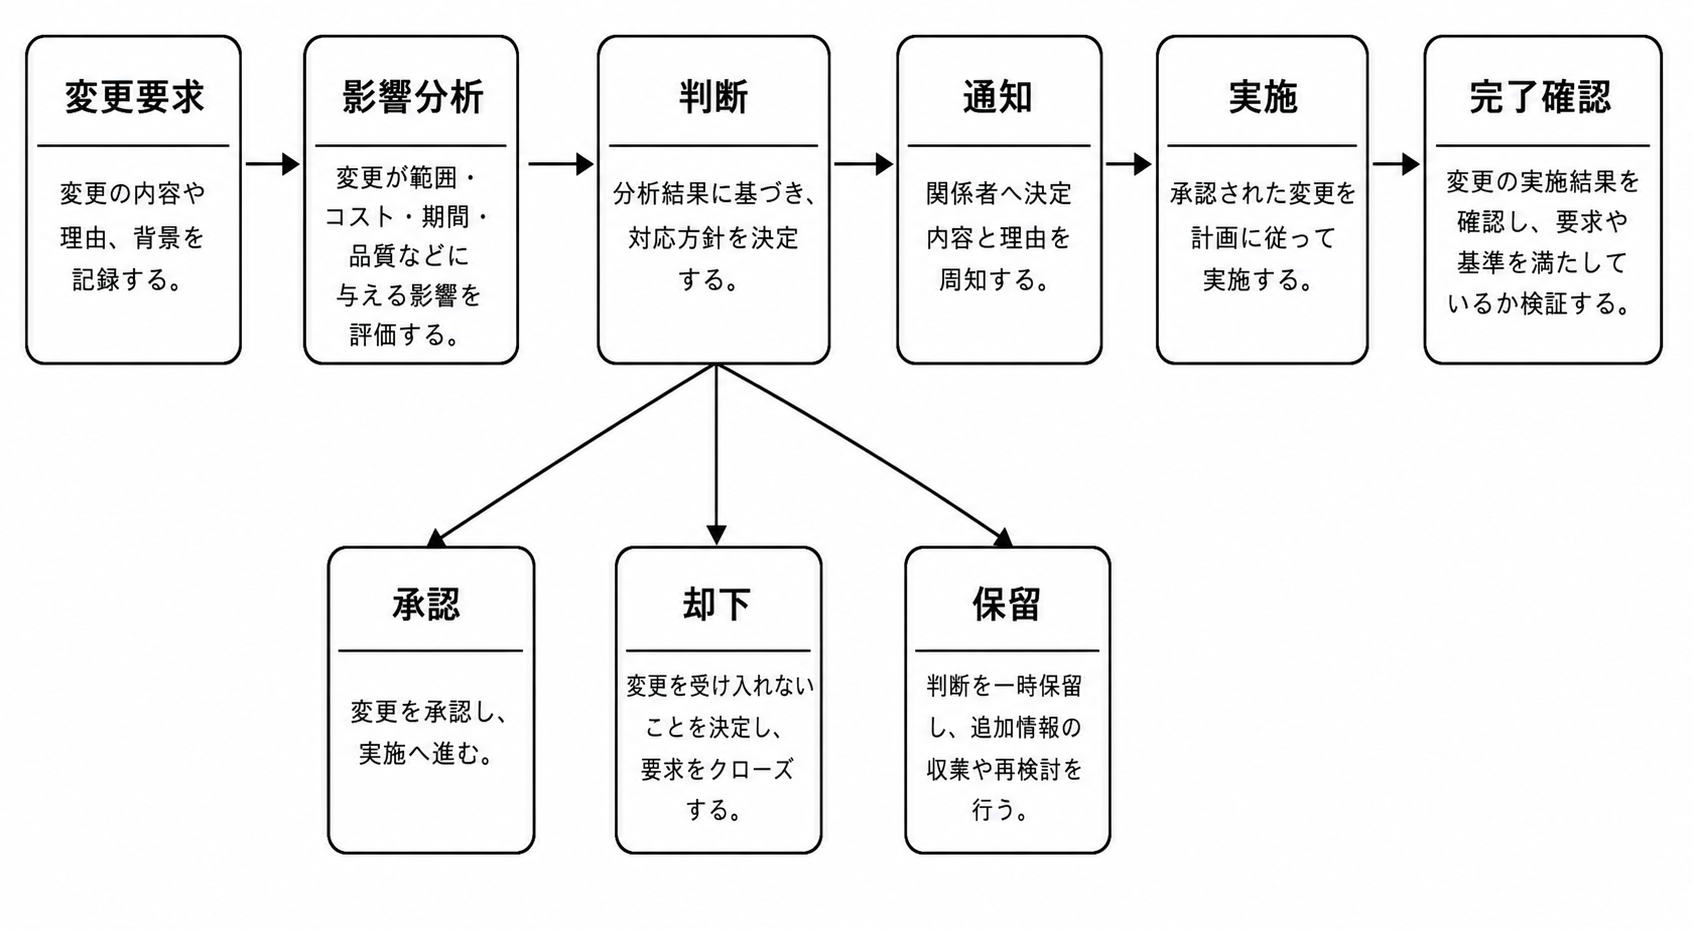
\includegraphics[width=0.96\linewidth]{assets/generated_figures/ch01/fig-ch01-10.png}}{\fbox{\parbox[c][48mm][c]{0.9\linewidth}{\centering 画像生成待ち\\要求変更管理の流れ}}}
\caption{要求変更管理の流れ}
\label{fig:ch01-10}
\end{figure}
